\part{Praktická část}

\hypertarget{analuxfdza-poux17eadavkux16f-na-aplikaci}{%
\chapter{Analýza požadavků na aplikaci}\label{analuxfdza-poux17eadavkux16f-na-aplikaci}}

V~praktické části této diplomové práce popisujeme výslednou webovou aplikaci pro geografické zmapování krajanských komunit a~jejich jazyka (dále jen aplikace). V~následujících kapitolách si ve stručnosti popíšeme související projekty, z~nichž jsme se při tvorbě více či méně inspirovali. Dále aplikaci představíme jak z~pohledu funkčních a~nefunkčních požadavků, tak z~hlediska návrhových a~implementačních částí.

\hypertarget{souvisejuxedcuxed-projekty}{%
\section{Související projekty}\label{souvisejuxedcuxed-projekty}}

XXX

\hypertarget{poux17eadavky-na-aplikaci}{%
\section{Požadavky na aplikaci}\label{poux17eadavky-na-aplikaci}}

Ještě před návrhovou fází vývoje je u~jakéhokoliv typu aplikace zapotřebí mít vyjasněny všechny požadavky, které jsou na daný systém kladeny. Tyto požadavky lze rozlišit na dva základny typy, a~to na funkční a~nefunkční.

\hypertarget{funkux10dnuxed-poux17eadavky}{%
\subsection{Funkční požadavky}\label{funkux10dnuxed-poux17eadavky}}

Funkční požadavky vyplývají z~účelu aplikace a~jsou typicky definované zákazníkem nebo jiným zadavatelem aplikace. Souvisí tak se základními funkcemi, akcemi a~aktivitami, jimiž by mělo digitální řešení disponovat pro řešení konkrétních problémů~\parencite{Gorton2006}.

Tyto požadavky můžeme u~naší webové aplikace pro větší přehlednost rozdělit do tří hlavních kategorií.

\hypertarget{geografickuxe1-reprezentace-ux10deskuxfdch-komunit-na-mapux11b}{%
\subsubsection{Geografická reprezentace českých komunit na mapě}\label{geografickuxe1-reprezentace-ux10deskuxfdch-komunit-na-mapux11b}}

Jedním z~nejdůležitějších nároků na aplikaci je vizualizace jednotlivých českých komunit po celém světě. Aplikace má tak disponovat samostatnou stránkou, v~rámci které budou dostupné mapové podklady celého světa. Na této mapě mají být pak prostřednictvím mapových vrstev vizualizovány konkrétní české enklávy. Pod mapovými vrstvami myslíme mnohoúhelníkové plochy, které mohou mít na mapě jakýkoliv tvar a~velikost podle potřeby vybrané komunity (geografická místa komunit v~aplikaci popisujeme jako lokality). Má být tak možné vizualizovat jak malé osady, tak celé regiony nebo státy -- vrstvy se též mohou jakýmkoliv způsobem překrývat.

Zapotřebí je také zahrnout základní funkční požadavky, které se pojí s~obsluhou mapové aplikace. Jde o~možnosti oddalování, a~přibližování pohledu (spolu s~navráceném do výchozí pozice), navigaci na mapě pomocí posouvání kurzoru klikání myší/dotykem anebo prostřednictvím minimapy zobrazující vždy širší kontext vybraného pohledu. Další důležitou mapovou funkcí je vyhledávání lokalit na mapě. Aplikace má umožňovat přiblížení na danou mapovou vrstvu na základě výběru ve vyhledávacím poli.

Zacílení lokalit má být umožněno i~jiným způsobem, než vyhledáváním v~mapových podkladech. Z~toho důvodu má aplikace disponovat výčtem lokalit, které budou dostupné z~mapové stránky prostřednictvím levé vysouvací části obrazovky. Tato sekce má sloužit jako přehledný abecedně seřazený seznam všech dostupných krajanských komunit (spolu s~úvodním obrázkem a~sekundárních názvem), z~něhož je možné lokalitu buď zacílit na mapě, anebo rovnou zobrazit její detail.

Posledním funkčním požadavkem souvisícím s~geografickou složkou je možnost filtrování lokalit na základě vybraných metrik (tyto metriky rozvedeme v~kapitole týkající se dat viz XXX). Tato funkce se má nacházet v~sekci se seřazenými komunitami a~po označení libovolného počtu filtrů se mají z~výběru i~z~mapových podkladů vyfiltrovat takové lokality, jež splňují danou podmínku.

\hypertarget{vizualizace-detailnuxedch-informacuxed-vybranuxe9-komunity}{%
\subsubsection{Vizualizace detailních informací vybrané komunity}\label{vizualizace-detailnuxedch-informacuxed-vybranuxe9-komunity}}

Druhým významným požadavkem na naši aplikaci je uživatelky přívětivá vizualizace všech dostupných informací, které se týkají vybrané krajanské komunity. Jelikož mohou být tyto informace rozličné velikosti a~multimediální povahy (audio soubory, obrázky, videa a~textové informace) je zapotřebí, aby v~aplikaci existoval sekundární navigační systém. Tato druhotná navigace má zajistit přehlednost při průchodu vybranou lokalitou a~umožnit tak uživateli výběr konkrétní části.

Jak bylo výše naznačeno, cílem našeho řešení je zmapovat ukázky komunikace v~češtině a~prostřednictvím audio nahrávek a~jejich transkriptů přiblížit jazyk dané české komunity. Požadavkem je tak také vhodné propojení audio souborů s~jejich přepisy.

Sekundárním požadavkem v~této oblasti je možnost sdílení vybrané lokality prostřednictvím URL adresy pro případnou kolaboraci při práci s~jednou určitou českou enklávou.

\hypertarget{administraux10dnuxed-prostux159eduxed-pro-editaci-jednotlivuxfdch-komunit}{%
\subsubsection{Administrační prostředí pro editaci jednotlivých komunit}\label{administraux10dnuxed-prostux159eduxed-pro-editaci-jednotlivuxfdch-komunit}}

Poslední kategorií jsou funkční požadavky spojené s~celkovou administrací jednotlivých komunit. Hlavní myšlenkou celé webové aplikace je otevřenost. A~to jak z~pohledu uživatele, který se chce dozvědět něco o~problematice (viz předchozí dvě kategorie), tak hlavně z~hlediska informované komunity, jež bude mít na starost přidávání nových lokalit, případě editaci či mazání již existujících oblastí.

Z~tohoto důvodu má aplikace obsahovat podstránky, které nebudou běžnému uživateli přístupné -- vzniká tak požadavek na autentifikaci prostřednictvím e-mailu a~hesla. Po úspěšném přihlášení by se měl celý systém přeměnit do editačního módu, respektive nabízet přihlášenému uživateli vždy kromě vstupu do jednotlivých lokalit i~možnost přesunu do administrativní části.

Ta by měla sestávat ze stejných sekcí, jako u~detailu vybrané komunity. Navíc by však by měla obsahovat uživatelsky přívětivou část formuláře podle formátu dané části informací (např. pro vkládání textových informací textový editor, pro vkládání souborů speciální komponentu). Druhotným požadavkem je pak základní validace vstupních data, tedy kontrola, že má každá lokalita vyplněný alespoň hlavní název a~geografická data pro zobrazení na mapě (viz xxx).

S~administrací tak nutně souvisí i~požadavek na persistenci dat, tzn. potřeba ukládat data na vzdálenou databázi, aby byly informace pro všechny uživatele konzistentní a~aktualizované.

\hypertarget{nefunkux10dnuxed-poux17eadavky}{%
\subsection{Nefunkční požadavky}\label{nefunkux10dnuxed-poux17eadavky}}

Pod nefunkčními požadavky si lze představit určitá omezení na design a~implementaci aplikace. Zde se jedná například o~volbu technologií, míru bezpečnosti, důraz na výkon či udržitelnost do budoucna atd. V~závěru se však vždy jedná o~určitý kompromis napříč jednotlivými faktory (např. vysoký výkon vs.~udržitelnost)~\parencite{Gorton2006}.

Hlavním nefunkčním požadavkem je, aby byl náš systém realizován jako webová aplikace, protože lze tak efektivně docílit k~multiplatformnímu výsledku. Z~tohoto faktu vyplývá potřeba responzivního řešení, tedy aby byla aplikace stejně funkční a~vzhledově atraktivní jak na zařízeních s~vyšším rozlišením, tak i~na menších obrazovkách. Dalším implicitním požadavkem je tím pádem i~nutnost internetového připojení.

Důležitou vlastností aplikace by také měla být udržitelnost a~rozšiřitelnost. V~tuto chvíli již existují konkrétní plány na rozšiřování aplikace mimo rozsah této diplomové práce, a~proto by měla být aplikace napsána se zásadami čistého a~čitelného kódu pro případné navázání jinými programátory.

\hypertarget{nuxe1vrh-aplikace}{%
\chapter{Návrh aplikace}\label{nuxe1vrh-aplikace}}

V~rámci představení návrhu aplikace se zaměříme na tři klíčová témata, jejichž obsah vychází především z~funkčních a~nefunkčních požadavků definovaných v~předchozí kapitole.

V~první části představíme použité technologie spolu s~odůvodněním jejich výběru. V~další podkapitole popíšeme strukturu a~obsah dat, ze kterých se skládají informace o~jednotlivých krajanských komunitách.

Hlavní součástí této kapitoly pak bude představení uživatelského rozhraní (UI) prostřednictvím konkrétních obrazovek aplikace. Zaměříme se zde také na popis interakce uživatele se systémem.

\hypertarget{pouux17eituxe9-technologie}{%
\section{Použité technologie}\label{pouux17eituxe9-technologie}}

Jelikož je naše navrhované řešení webová aplikace, budeme se níže zabývat výhradně nástroji, knihovnami a~frameworky, které se primárně týkají webových technologií. Konkrétní příklady kódu budeme rozebírat v~kapitole týkající se vlastní implementace (viz xxx).

\hypertarget{zuxe1kladnuxed-webovuxe9-technologie}{%
\subsection{Základní webové technologie}\label{zuxe1kladnuxed-webovuxe9-technologie}}

I~přes to, že je svět webových technologií jednou z~nejdynamičtěji rozvíjejících se oblastí IT, jeho základy jsou již několik desítek let stále stejné. Aby mohl webový prohlížeč vykreslit (renderovat) webovou stránku\footnote{Pojmy webová stránka a~webová aplikace vnímáme v~tomto kontextu totožně. Tedy vše, co platí pro vývoj webových stránek, platí i~pro vývoj webových aplikací (protože aplikace jsou v~principu jen komplexnější formou webových stránek).}, musí být její obsah vždy určitým způsobem strukturovaný. Pro tyto účely se již řadu let využívá HTML (Hypertext Markup Language) -- značkovací jazyk, který popisuje přesnou strukturu určitého dokumentu.

Prostřednictvím značek tohoto jazyka dáváme jednotlivým částem dokumentu strukturální významy. Mohou to být například značky pro označení odstavce, odkazů nebo třeba tabulek či videí. Některé značky sice mohou vyvolat změny vzhledu dané části dokumentu, nicméně pro tyto účely HTML není primárně určeno~\parencite{htmlcss}.

Abychom mohli upravit vzhled webové stránky, je zapotřebí využít druhé základní technologie, a~to CSS (Cascading Style Sheets). Jedná se o~jazyk, pomocí kterého lze konkrétním HTML značkám přiřazovat předdefinované vlastnosti, a~tak jim měnit vzhled dle potřeb. Typicky může jít o~změny barvy, velikosti, fontů, ale i~třeba o~implementaci složitějších animací, přechodů atd.~\parencite{htmlcss}.

HTML a~CSS lze od sebe izolovat do dvou či více separátních souborů, což je standardní způsob jak efektivně oddělit vizuální složku od strukturální.

Třetí základní technologií je programovací jazyk JavaScript (oficiálně ECMAscript), který předchozí dvě složky doplňuje o~možnost interakce uživatele s~webovou stránkou. JavaScript je skriptovací jazyk, který není narozdíl od jiných programovacích jazyků typu Java nebo Objective-C zapotřebí před spuštěním kompilovat (stačí tedy pro jeho použití využít jakýkoliv z~dostupných webových prohlížečů). Díky této technologii lze dynamicky upravovat obsah webové stránky, to znamená že JavaScript využijeme především v~situacích, kdy od uživatele očekáváme nějakou aktivitu (např. stisknutí tlačítka nebo klávesy atd.)~\parencite{javascript}.

Aby JavaScript a~CSS mohly přistupovat k~jednotlivým částem HTML, dochází vždy před vykreslením k~převedení ze značkovacího jazyka do takzvaného DOM (Document Object Model). Jedná se o~objekt stromové struktury, v~němž je uložené vlastní HTML a~každá značka (uzel) si drží informaci o~své lokaci. CSS pak na tento objekt aplikuje svá pravidla pro správné vykreslení a~JavaScript případně mění strukturu spolu s~další části tohoto stromového objektu~\parencite{howbrowserswork}.

\hypertarget{pux159uxedstupy-k-vykreslovuxe1nuxed-webovuxfdch-struxe1nek}{%
\subsection{Přístupy k~vykreslování webových stránek}\label{pux159uxedstupy-k-vykreslovuxe1nuxed-webovuxfdch-struxe1nek}}

Při výběru dalších technologií pro vývoj webové aplikace si je zapotřebí nejdříve uvědomit, jakou strategii vykreslování bude naše aplikace naplňovat.

\hypertarget{dynamickuxe9-webovuxe9-struxe1nky}{%
\subsubsection{Dynamické webové stránky}\label{dynamickuxe9-webovuxe9-struxe1nky}}

Jednou z~nejčastějších strategií je dynamické vykreslování stránek. Jedná se o~princip, kdy je webová stránka (tedy HTML s~CSS a~JavaScriptem) se všemi potřebnými informacemi dynamicky vytvořena na vzdáleném serveru. Prohlížeč (jinými slovy klient) tak na základě akce od uživatele pošle na server takzvaný \emph{request} a~server vygenerovanou webovou stránku obratem pošle nazpět.

Výhodou toho přístupu je fakt, že klient dostane už kompletní dokument se všemi potřebnými informacemi (což je výhodné z~hlediska SEO\footnote{Search engine optimization (SEO) je proces optimalizace viditelnosti webových stránek v~rámci internetových vyhledávačů jako je např. Google. Čím lepší je SEO, tím je pravděpodobnější, že se daná webová stránka objeví na vyšších příčkách při vyhledávání.}). Neméně důležitým přínosem je pak to, že se veškerá logika děje na serveru (který je typicky výkonnější než klient, prohlížeč akorát vykresluje výsledek.

Na druhou stranu lze vidět i~nevýhodu primárně v~opakovaném generování každé stránky při opětovné návštěvě, což může být problém při pomalejším internetovém připojení. Komplikovanější též může být vývoj samotných aplikací, protože vývojář musí znát jak HTML, CSS a~JavaScript (souhrnně frontend), tak technologie spojené se serverovou částí (práce s~databází atd.). protože jsou na sebe obě složky na serveru nutně navázané~\parencite{spa}.

\begin{figure}[ht]   
    \centering
    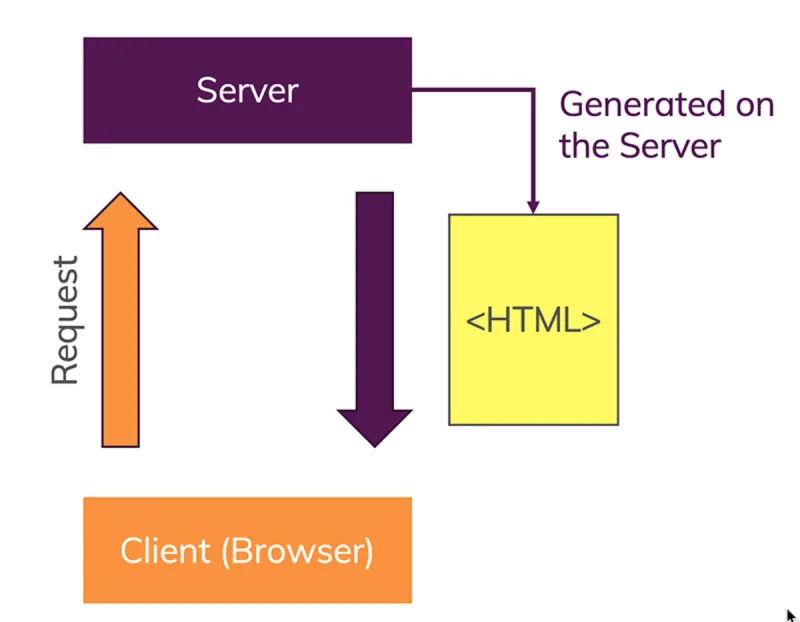
\includegraphics[width=.5\textwidth]{dynamic}  
    \caption{Dynamické vykreslování}
    \label{dynamic}
 \end{figure}

\hypertarget{statickuxe9-webovuxe9-struxe1nky}{%
\subsubsection{Statické webové stránky}\label{statickuxe9-webovuxe9-struxe1nky}}

Druhý přístup je nejstarší a~zároveň nejjednodušší, protože se jedná o~již vytvořené HTML (spolu s~CSS a~JavaScriptem) soubory, které jsou neměnné. To znamená, že jsou tyto již připravené statické soubory uložené na serveru, kde očekávají request od klienta k~vykreslení. Jedná se tedy nejčastěji o~takové webové stránky, které jsou jednodušší a~neočekává se u~nich příliš mnoho interaktivity s~uživatelem.

V~dnešní době jsou navíc populární takzvané generátory statických stránek, které umožňují vytvářet statické stránky na základě předpřipravených šablon a~odlehčeného značkovacího jazyka jako je například Markdown\footnote{https://www.markdownguide.org/}, v~němž se vytváří samostatný obsah~\parencite{spa}.

\begin{figure}[ht]   
    \centering
    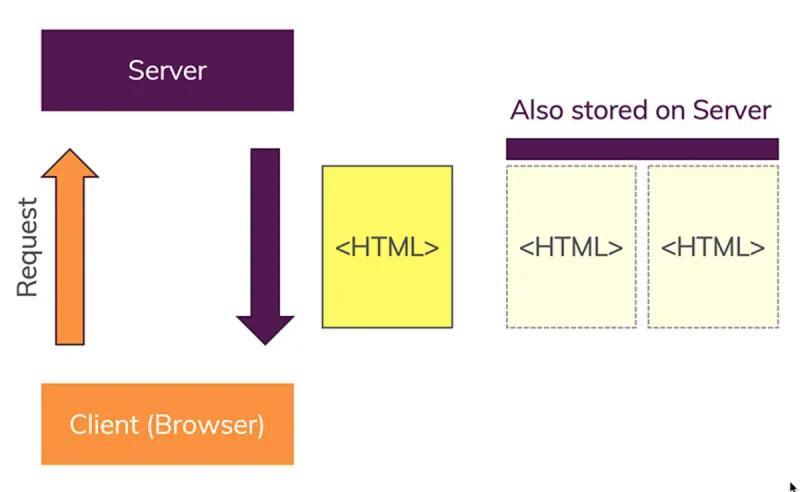
\includegraphics[width=.5\textwidth]{static}  
    \caption{Statické vykreslování}
    \label{static}
 \end{figure}

\hypertarget{single-page-applications}{%
\subsubsection{Single Page Applications}\label{single-page-applications}}

Posledním populárním přístupem jsou takzvané Single Page Applications (SPA), jejichž princip je přesně opačný od dynamických webových stránek. Klient sice také musí poslat request na server, nicméně ten vrací vždy jeden stejný HTML soubor s~velkým množství přidruženého javaScriptového kódu. JavaScript pak v~prohlížeči upravuje samotný DOM HTML souboru do výsledné podoby pro vykreslení.

Díky této strategii jsou webové stránky tohoto typu vysoce uživatelsky přívětivé, protože se veškeré vizuální změny dějí na klientovi. Pokud je tedy zapotřebí například stáhnout data z~databáze, JavaScript změní DOM do určité formy vizuálně přívětivého načítání nebo umožní data stahovat v~pozadí a~uživatel se může v~aplikace dál pohybovat. V~předchozích případech případech by návštěvník webu musel čekat, až se všechny změny provedou na serverové části.

Tento přístup má dvě základní nevýhody. Zaprvé může být v~některých případech pro prohlížeč náročné zpracovat všechny javaScriptové instrukce pro vygenerování výsledného HTML (zvláště, pokud jsou SPA neefetkivně napsané nebo uživatel používá starší zařízení / má pomalejší připojení). Druhým problémem bývá již zmíněné SEO -- iniciální HTML soubor totiž obsahuje malé množství metadat a~dalších informací o~stránce (jelikož ještě neproběhlo generování JavaScriptem) a~pro prohlížeč se webová stránka nemusí jevit důvěryhodně a~přiřazuje ji tak menší váhu při vyhledávání~\parencite{spa}.

\begin{figure}[ht]   
    \centering
    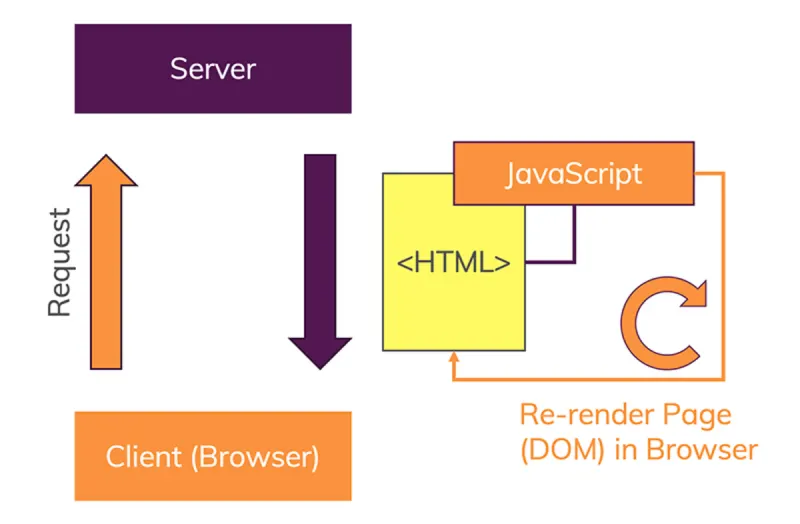
\includegraphics[width=.5\textwidth]{spa}  
    \caption{Single Page Application}
    \label{spa}
 \end{figure}

Jelikož naše aplikace obsahuje komplexnější komponenty, které nebývají součástí základních webových stránek (např. mapa pro geografické zobrazování), a~počítá s~vyšší mírou uživatelské interakce (např. administrační prostředí spolu s~autentifikací), volíme právě tento přístup pro vývoj našeho řešení.

\hypertarget{react}{%
\subsection{React}\label{react}}

Jak bylo výše napsáno, vývoj SPA aplikací je především záležitostí programování javaScriptového kódu. Aby nemuseli vývojáři veškerou integraci a~tvorbu základních funkcionalit tvořit stále od začátku, existují takzvané webové frameworky. Jejich hlavní význam je zjednodušit a~zefektivnit vývoj uživatelského rozhraní (frameworky samozřejmě existují i~pro ostatní části vývoje, například pro backend atd.) a~nastavují tak daným komunitám vývojářů základní pravidla, a~tím pádem určitou konzistenci pro strukturalizaci kódu. Tento aspekt je zvláště důležitý, pokud na určitém projektu pracuje větší množství lidí.

V~našem případě byly jedním z~nejdůležitějších nefunkčních požadavků udržitelnost a~rozšiřitelnost. Proto za webový framework vybíráme React\footnote{I přes to, že v~našem textu React popisujeme jako webový framework, není tomu zcela tak. Zcela přesně se jedna o~webovou knihovnu, která má mírně odlišné charakteristiky (např. výkon, komplexita atd.), nicméně pro naše účely můžeme tyto významové nuance ignorovat.}, který je v~tuto chvíli stále nejpopulárnější volbou mezi vývojáři na celém světě\footnote{https://www.developer-tech.com/news/2021/aug/03/2021-stack-overflow-survey-react-js-takes-the-web-framework-crown-python-is-in-demand-and-devs-still-love-rust/} a~základní znalost tohoto nástroje je tak v~dnešní době pro webové vývojáře takřka podmínkou.

Jedná se o~open-source software\footnote{https://github.com/facebook/react} vytvořený v~roce 2013 a~udržovaný programátory společností Meta (dříve Facebooku) za podpory široké komunity vývojářů~\parencite{react}.

React je založen na deklarativním vývoji uživatelského rozhraní. Vývojář tedy vytváří vzhled pro všechny stavy aplikace, které se pak vykreslují na základě změny v~datech (např. u~přihlášeného uživatele není zapotřebí zobrazovat tlačítko přihlášení a~naopak). Kód je tak pochopitelnější a~jednodušší na ladění chyb (debugging).

Druhou významnou vlastností Reactu je přístup založený na komponentách. Jedná se o~opakovaně použitelné části UI (tzn. i~samotného naprogramovaného kódu), které jsou hierarchicky strukturované buď podle využití v~aplikaci (např. adresář s~komponentou pro přihlášení \emph{Login} bude obsahovat soubor podkomponenty pro tlačítko \emph{LoginButton}), nebo podle obecně sdílených funkcionalit (všechny komponenty tlačítek v~aplikaci budou ve vlastní složce \emph{Buttons}). Data, na kterých jsou závislé jednotlivé stavy, lze mezi komponentami předávám prostřednictvím objektu s~názvem \emph{props}.

React namísto klasického stromové objektu DOM (viz XXX) využívá koncept virtuálního DOM (virtual Document Object Model). Jedná se o~speciální objektovou strukturu uloženou v~mezipaměti prohlížeče, která umožňuje efektivněji synchronizovat změny v~UI s~daným stavem aplikace. Zjednodušeně řečeno jde o~odlehčenou verzi DOM, s~níž je na úrovni klienta jednodušší na úrovni klienta manipulovat a~přizpůsobovat akcím od uživatele.

Posledním důležitým specifikem tohoto webového frameworku je využívání jazyka JSX, který je doporučován pro zápis komponent. JSX je svojí syntaxí nadstavbou JavaScriptu a~kombinuje strukturní značky, které známe z~HTML s~javaScriptovými konstrukcemi pro práci s~proměnnými a~funkcemi/metodami.

\hypertarget{typescript}{%
\subsection{TypeScript}\label{typescript}}

V~předchozí podkapitolách jsme popisovali významnou roli JavaScriptu při vývoji webových aplikací, nicméně existuje modernější a~vhodnější varianta tohoto programovacího jazyka -- TypeScript. Nejedná se ale o~nový, samostatný jazyk, ale o~rozšíření syntaxe stávajícího JavaScriptu. TypeScript byl vytvořen v~roce 2012 společností Microsoft a~jeho hlavním cílem je obohatit JavaScript o~typovou kontrolu objektů a~proměnných. Pomocí typové kontroly lze docílit k~větší prevenci potenciálních chyb a~celý kód se tak navíc stává přehlednějším~\parencite{typescript}.

Jelikož se chceme držet zásad čitelného a~čistého kódu, použijeme TypeScript i~v~naší aplikaci. Zároveň je zapotřebí dodat, že je javaScriptová syntaxe podmnožinou TypeScriptu\footnote{Typescript se vždy před spuštěním nejprve převede do čistého JavaScriptu, proto lze v~TypeScriptu psát v~případě potřeby čistý javaScriptový kód.}, tedy pro TypeScript platí všechny informace, které se v~této práci vážou k~JavaScriptu.

\hypertarget{technologie-spojenuxe9-s-vizualizacuxed-komunit-na-mapux11b}{%
\subsection{Technologie spojené s~vizualizací komunit na mapě}\label{technologie-spojenuxe9-s-vizualizacuxed-komunit-na-mapux11b}}

Hlavní součástí aplikace je vizualizace jednotlivých českých komunit po celém světě. Mapovými podklady (spolu s~nástroji, které s~mapou manipulují) standardně webové frameworky nedisponují. Níže popisujeme technologie, které jsme vybrali a~integrovali do našeho řešení.

\hypertarget{openstreetmap}{%
\subsubsection{OpenStreetMap}\label{openstreetmap}}

Za mapové podklady jsme vybrali volně editovatelné a~otevřené topografické mapy OpenStreetMap. Jedná se o~projekt, který vznikl v~roce 2004 jako protiváha proti tehdejším proprietárním řešením. Byl inspirován úspěchem wikipedie a~jeho cílem je distribuovat volně dostupná geografická data jak pro nekomerční, tak komerční účely~\parencite{open-street}. Z~těchto důvodu jsme OpenStreetMap vybrali i~do naší aplikace.

\hypertarget{leaflet}{%
\subsubsection{Leaflet}\label{leaflet}}

Pro manipulaci s~OpenStreetMap jsme využili open-source javaScriptovou knihovnu Leaflet\footnote{Autorem knihovny je Kyjevan Volodymyr Agafonkin, který kvůli ruské invazi v~roce 2022 stejně jako mnoho ostatních Ukrajinců utekl ze svého domova. Téma této práce se týká i~nucených emigrací, a~proto si zde dovolíme udělat menší vložku a~vepsat odkaz, kde je možné podpořit Ukrajinu v~této nelehké době – https://www.comebackalive.in.ua/.}. Tento nástroj umožňuje webovým vývojářům vizualizovat na mapových podkladech vlastní interaktivní značky, vrstvy a~další vizuální prvky bez znalosti GIS\footnote{https://education.nationalgeographic.org/resource/geographic-information-system-gis}~\parencite{leaflet}.

Integrace nástroje Leaflet do frameworku React jsme provedli prostřednictvím knihovny React Leaflet. Ta je nástavbou předchozí knihovny a~abstrahuje jednotlivé složky Leafletu do systému komponent a~stavů, které jsou typické pro React~\parencite{react-leaflet}.

\hypertarget{geojson}{%
\subsubsection{GeoJSON}\label{geojson}}

Abychom byli schopni vkládat do OpenStreetMap prostřednictvím Leafletu vlastní geografická data krajanských komunit, musíme zvolit vhodný formát dat. Přenos dat ve světě webových technologií standardně probíhá pomocí formátu JSON (JavaScript Object Notation). Jde o~otevřený standard pro výměnu dat, který používá čitelný zápis skládající se vždy z~dvojic klíč -- hodnota. I~přes to, že je použitelný napříč programovacími jazyky, vychází z~JavaScriptu, konkrétně ze zápisu objektů (což je výhodné, protože se dá z~dat ihned vytvořit objekt a~dále s~nimi pracovat jako s~proměnnou). Jeho použití je rozmanité, nicméně se s~ním lze nejčastěji setkat při komunikaci mezi webovými aplikacemi a~vzdálenými servery~\parencite{json}.

GeoJSON z~formátu JSON vychází -- jedná se tedy o~otevřený standard pro reprezentaci takzvaných \emph{features} (OpenGIS standard pro specifikaci geografických dat). Pod \emph{features} si můžeme představit konkrétní tvary na mapě jako jsou například body, čáry, ale hlavně mnohoúhelníky, které využíváme pro vizualizaci lokalit~\parencite{geojson}.

Detailní tvorba \emph{features} ve formátu GeoJSON může být v~textovém editoru komplexní a~časově náročnou aktivitou. Jelikož je našim cílem editovat lokality v~aplikaci uživatelsky přívětivým způsobem, využíváme externí službu Geoman.io, která disponuje již vytvořeným GeoJSON editorem~\parencite{geoman}.

\hypertarget{firebase}{%
\subsection{Firebase}\label{firebase}}

Z~funkčních požadavků dále vyplývá potřeba ukládat data na vzdálenou databázi, aby byly informace pro všechny uživatele konzistentní a~aktualizované. Pro naplnění tohoto nároku jsme se rozhodli vybrat platformu Firebase od firmy Google, která nabízí předpřipravená cloudová řešení pro backendovou část (správa databáze a~autentifikace atd.) mobilních a~webových aplikací~\parencite{firebase}. Pro naše potřeby jsme využili tři nástroje popsané níže.

\hypertarget{firebase-authentication}{%
\subsubsection{Firebase Authentication}\label{firebase-authentication}}

Firebase Authentication je služba, která poskytuje komplexní řešení autentifikace v~souladu se základními standardy jako jsou OAuth 2.0 and OpenID. Výhodou tohoto řešení je její integrace i~do ostatních Firebase produktů, je tedy možné např. nastavovat práva pro konkrétní přihlášené/nepřihlášené uživatele týkající se zápisu do Cloud Firestore databáze.

Nástroj nabízí registraci a~přihlašování přes různé poskytovatele jako jsou Facebook, Google anebo Twitter, my ale využíváme klasického přihlášení přes e-mail a~heslo. V~této verzi aplikace nemá uživatel možnost vlastní registrace, protože administrační část je otevřena pouze ověřeným editorům krajanských komunit~\parencite{auth}.

\hypertarget{cloud-firestore}{%
\subsubsection{Cloud Firestore}\label{cloud-firestore}}

Druhým využitým nástrojem je Cloud Firestore -- databázové řešení, v~němž ukládáme všechna data textové povahy. Jedná se flexibilní a~škálovatelnou dokumentovou databázi, která ukládá data do kolekcí a~izolovaných JSON dokumentů (tzn. uložená data jsou až na pár detailů velmi podobná formátu, který využíváme v~naší aplikaci). Tuto databázi využíváme jako hlavní uložiště pro jednotlivé lokality~\parencite{firestore}.

\hypertarget{cloud-storage}{%
\subsubsection{Cloud Storage}\label{cloud-storage}}

Poslední zvolenou službou je Cloud Storage. Jde o~jednoduché a~cenově výhodné cloudové uložiště, které je uzpůsobeno k~ukládání netextových souborů jako jsou obrázky, audio soubory či videa. Tento nástroj umožňuje efektivní stahování a~nahrávání větších souborů spolu s~jejich validací a~kontrolou existence. Taktéž je navázán na Firebase Authentication a~lze tak regulovat přístup k~některým souborům. Výhodou tohoto řešení je vysoká míra škálovatelnosti, kterou je zapotřebí řešit při větším počtu aktivních uživatelů~\parencite{storage}.

\hypertarget{data-o-krajanskuxfdch-komunituxe1ch}{%
\section{Data o~krajanských komunitách}\label{data-o-krajanskuxfdch-komunituxe1ch}}

Jelikož jsou data nutnou součástí a~vlastně i~samotným smyslem aplikace, popisujeme v~následující podkapitole strukturu a~obsah dat, ze kterých se skládají informace o~jednotlivých krajanských komunitách.

Zároveň platí, že všechny zmíněné složky lze v~administrativní části upravovat. Kromě názvu hlavní lokality a~geografických dat není žádná z~položek povinná, protože u~každé komunity nemusí být dostupné všechny typy informací. Pro větší přehlednost tyto informace dělíme do podsekcí tak, jak je lze najít v~administraci webové aplikace.

\hypertarget{uxfavod}{%
\subsection{Úvod}\label{uxfavod}}

\begin{itemize}
\tightlist
\item
  \textbf{Název hlavní lokality} -- jedná se o~unikátní název, bez kterého nelze lokalitu vytvořit. Podle tohoto hlavního názvu je komunit tříděna v~seznamu komunit lokalit;
\item
  \textbf{Název sekundární lokality } -- doplňující název pro vyšší správní jednotky, tedy pro region, kraj nebo stát;
\item
  \textbf{Úvodní obrázek} -- náhledový obrázek, kterým je lokalita znázorněna ve vedlejším seznamu, anebo při rozkliku mapové vrstvy;
\item
  \textbf{Demografické údaje} -- základní údaje, týkající se především demografie komunity. Taktéž jsou zde pro větší přehlednost vypsány hodnoty, podle kterých mohou být aplikovány filtry (viz xxx).
\end{itemize}

\hypertarget{detailnuxed-informace}{%
\subsection{Detailní informace}\label{detailnuxed-informace}}

\begin{itemize}
\tightlist
\item
  \textbf{Nahrávka}

  \begin{itemize}
  \tightlist
  \item
    Audio nahrávka -- audio soubor s~nahrávkou, která obsahuje příklad autentického jazyka vybrané české komunity;
  \item
    Název nahrávky a~případný komentář ke vzniku -- název audio nahrávky s~případným doprovodný komentářem;
  \item
    Přepis nahrávky -- fonetická transkripce zvukové nahrávky do textové podoby (bez použití speciálních znaků);
  \item
    Poznámky k~jazyku a~jazyková charakteristika -- komentář k~jazyku nahrávky a~popis jazykové charakteristiky komunity (hláskosloví, tvarosloví atd.);
  \item
    Další zdroje -- prostor pro odkazy na jazykovou normu či jiné zdroje.
  \end{itemize}
\item
  \textbf{Historie a~současnost}

  \begin{itemize}
  \tightlist
  \item
    Historie -- sekce určená k~popisu historie komunit;
  \item
    Současnost -- text věnovaný k~aktuálnímu stavu české enklávy.
  \end{itemize}
\end{itemize}

\hypertarget{multimediuxe1lnuxed-obsah}{%
\subsection{Multimediální obsah}\label{multimediuxe1lnuxed-obsah}}

\begin{itemize}
\tightlist
\item
  \textbf{Autor fotografií/obrázků} -- jméno a~a~případně odkaz na autora obrázků a~fotografií;
\item
  \textbf{Obrázky} -- libovolné množství fotografií a~dalších ilustračních obrázků dané české komunity spolu s~krátkými popisky;
\item
  \textbf{Audio} -- libovolné množství audio nahrávek s~rozhovory s~krajany či odborníky na danou lokalitu (spolu s~krátkými popisky);
\item
  \textbf{Videa} -- libovolné množství odkazů na videa o~komunitě spolu s~popisky;
\item
  \textbf{Texty} -- prostor na ukázky textových materiálů jako jsou úryvky z~knih, místních časopisů atd.;
\item
  \textbf{Ostatní} -- sekce na doplňující informace, které se nehodily umístit nikam jinam.
\end{itemize}

\hypertarget{ostatnuxed}{%
\subsection{Ostatní}\label{ostatnuxed}}

\begin{itemize}
\tightlist
\item
  \textbf{Projekty} -- informace o~existujících projektech související s~vybranou lokalitou;
\item
  \textbf{Nabídky} -- vyjmenování případných nabídek spolupráce či jiných participací s~komunitou;
\item
  \textbf{Atrakce} -- doplňující informace týkající se lokálních atrakcí, přírodních památek nebo turistického vyžití na daném místě;
\item
  \textbf{Zajímavosti} -- dodatečné zajímavosti ohledně historie, demografie či tamější architektury atd.;
\item
  \textbf{Zdroje} -- prostor na vkládání všech zdrojů, jež byly využity pro tvorbu digitálního záznamu o~krajanské komunitě;
\item
  \textbf{Kontakt} -- kontakt na tvůrce konkrétního záznamu.
\end{itemize}

\hypertarget{geografickuxe1-data}{%
\subsection{Geografická data}\label{geografickuxe1-data}}

\begin{itemize}
\tightlist
\item
  \textbf{GeoJSON} -- pole pro vkládání jedné mapové vrstvy ve formátu GeoJSON. Na tomto místě je také příložen odkaz na službu Geoman.io, prostřednictvím které lze jednoduše kreslit jednotlivé mapové objekty a~generovat tak GeoJSON soubor;
\item
  \textbf{Podmínky pro třídění na mapě} -- všechny níže uvedené podmínky jsou ve formě polí výběru (selection box), u~nichž lze vybírat libovolné množství hodnot (níže je vždy vedle názvu filtru vypisujeme). Podle těchto vybraných hodnot je pak možné lokality filtrovat na mapě a~v~bočním seznamu;

  \begin{itemize}
  \tightlist
  \item
    Doba příchodu česky mluvících osob

    \begin{itemize}
    \tightlist
    \item
      1550--1620,
    \item
      1620--1700,
    \item
      1700--1800,
    \item
      1800--1850,
    \item
      1850--1914,
    \item
      1914--1930,
    \item
      po 1939,
    \item
      po 1989;
    \end{itemize}
  \item
    Doba zániku

    \begin{itemize}
    \tightlist
    \item
      před 1620,
    \item
      před 1700,
    \item
      v~18. století,
    \item
      v~19. století,
    \item
      v~1. pol. 20. stol,
    \item
      ve 2. pol. 20. stol,
    \item
      2000--současnost;
    \end{itemize}
  \item
    Velikost komunity

    \begin{itemize}
    \tightlist
    \item
      méně než 10,
    \item
      10--50,
    \item
      více než 50,
    \item
      více než 500,
    \item
      více než 10 000,
    \item
      více než 50 000;
    \end{itemize}
  \item
    Převládající nářeční základ

    \begin{itemize}
    \tightlist
    \item
      městská mluva,
    \item
      severovýchodočeská skupina,
    \item
      středočeská,
    \item
      jihozápadněčeská skupina,
    \item
      středomoravská,
    \item
      východomoravská,
    \item
      lašská,
    \item
      českomoravská;
    \end{itemize}
  \item
    Počet generací, po které se čeština uchovala

    \begin{itemize}
    \tightlist
    \item
      1,
    \item
      2,
    \item
      3,
    \item
      4,
    \item
      5,
    \item
      6,
    \item
      7,
    \item
      8,
    \item
      9,
    \item
      10;
    \end{itemize}
  \item
    Převládající motivace pro emigraci z~českých zemí

    \begin{itemize}
    \tightlist
    \item
      náboženská (cca do 1850),
    \item
      hospodářská (1820--1939, po 1989),
    \item
      politická (zejm. po 1939--1989);
    \end{itemize}
  \item
    Existuje audiomateriál nebo písemná dokumentace jazyka?

    \begin{itemize}
    \tightlist
    \item
      ano,
    \item
      ne;
    \end{itemize}
  \item
    Převládající náboženství

    \begin{itemize}
    \tightlist
    \item
      protestantské,
    \item
      katolické,
    \item
      bez vyznání,
    \item
      nezjištěno;
    \end{itemize}
  \item
    Proběhla reemigrace?

    \begin{itemize}
    \tightlist
    \item
      po 1. světové válce,
    \item
      po 2. světové válce;
    \end{itemize}
  \item
    Typ migrace

    \begin{itemize}
    \tightlist
    \item
      primární,
    \item
      sekundární,
    \item
      další migrace.
    \end{itemize}
  \end{itemize}
\end{itemize}

\hypertarget{uux17eivatelskuxe9-rozhranuxed}{%
\section{Uživatelské rozhraní}\label{uux17eivatelskuxe9-rozhranuxed}}

V~této podkapitole představíme

\begin{figure}[hb!]   
    \centering
    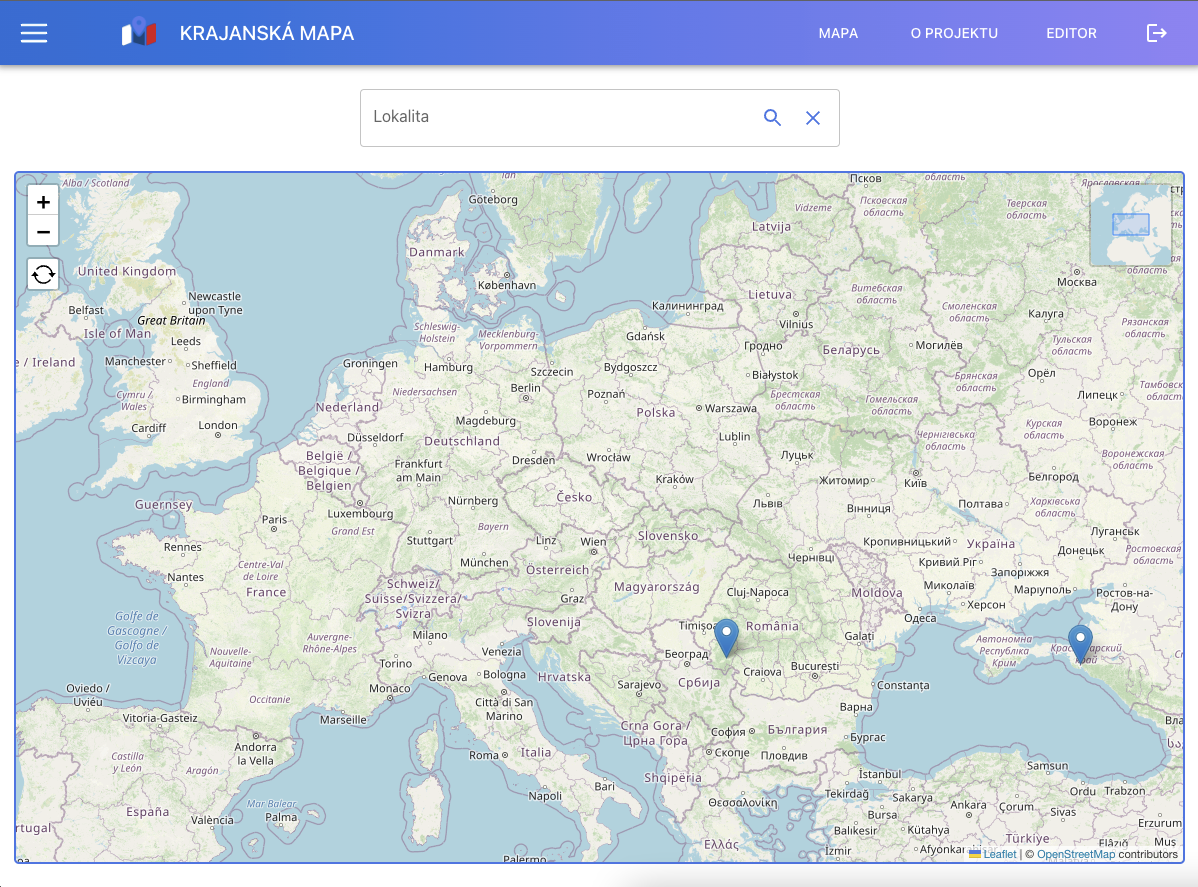
\includegraphics[width=0.95\textwidth]{mapa}  
    \caption{Výchozí pohled na mapu}
    \label{mapa}
\end{figure}

\hypertarget{responzivnuxed-design}{%
\subsection{Responzivní design}\label{responzivnuxed-design}}
